\documentclass[10pt]{article}

\usepackage[hmarginratio=1:1,top=32mm,columnsep=20pt]{geometry}                 \usepackage{booktabs}     	
\usepackage{graphicx}
\usepackage{subcaption}
\usepackage[backend=bibtex,sorting=none]{biblatex}
\usepackage{hyperref}
\hypersetup{colorlinks=true,
            urlcolor=blue}
	    
\bibliography{references}

\title{Healthcare Data Lake}

\author{
	\textsc{Kendal, Joseph}\\
	\normalsize University of Bristol\\
	\texttt{jk17246@bristol.ac.uk}
	
	\and
	
	\textsc{Sherred, Jago}\\
	\normalsize University of Bristol\\
	\texttt{j.sherred.2019@bristol.ac.uk}
	
	\and
	
	\textsc{Benson, Luke}\\
	\normalsize University of Bristol\\
	\texttt{wr19606@bristol.ac.uk}
	
	\and
	
	\textsc{Liu, Anna}\\
	\normalsize University of Bristol\\
	\texttt{gf19916@bristol.ac.uk}
	
	\and
	
	\textsc{Cismaru, Armand}\\
	\normalsize University of Bristol\\
	\texttt{fz19792@bristol.ac.uk}
}


\begin{document}

\maketitle    


\begin{abstract}

Digital healthcare provided by the NHS in England typically operates in silos. GPs have electronic systems to manage patient care which are distinct from hospital systems which are distinct from the ambulance service, 111, mental health services etc. Each data owner has a wealth of data that, if combined, would generate a more valuable resource than it does in isolation. While there are solutions to integrate this data for direct care purposes, there is no centralised solution to use this data to inform future care or service provisioning. This project is designed to explore the benefits of cloud technologies to produce a prototype secure, scalable health data storage platform that can underpin local healthcare analytics.

\end{abstract}

\section{Overview}
%TODO%

\subsection{Client}
Dr. Philip D Harfield, Health Data Scientist (Informatics) at NIHR Bristol Biomedical Research Centre, University of Bristol.
\subsection{Domain}
The domain of our Healthcare Data Lake project is the Healthcare Analytics Environment team who will design, implement and test a set
of candidate cloud-hosted analytics environments that provide sufficient functionality while also maintaining a secure data environment.
\\
The overall domain of the three teams is NHS Healthier Together Sustainability Transformation Partnership Bristol, North Somerset, and South Gloucestershire (BNSSG) \& Bristol Biomedical Research Centre, University of Bristol Medical School.
\subsection{Project}
The project entails combining a wealth of data from data owners(GPs Patient data, ambulance services, 111, mental health services .etc) into a data lake. This will be used to inform clinical decisions making by providing more advanced insights into the longitudinal health of the patient on arrival and understand the merits of previous clinic decisions taken.
\\
The project will explore the benefits of cloud technologies and produce a prototype secure, scalable health data storage platforms that can underpin local healthcare analytics.
\\
The project is one of three designed an end-to-end proof of concept to the local NHS. We will be working alongside the "Healthcare Data Visualisation" and "Healthcare Analytics Environment" teams. 
\subsection{Vision}
The Healthcare Data Lake Project is envisioning a future integrated data storage solution, one that is scalable and portable, while using the latest cloud-based technologies. Starting with a prototype, the final scope is to create, alongside the Simulation and Analytics Projects, a system that is going to change how data is handled and used in the healthcare system. There is the real possibility that this three projects will represent the cornerstone of a future solution used and developed extensively by the NHS, which will bring immediate aid to the average medical worker and improve the quality of the service provided to the patients.

\newpage


\section{Stakeholder and Requirements
Analysis}\label{stakeholder-and-requirements-analysis}

\subsection{Primary Stakeholder and User
Story}\label{primary-stakeholder-and-user-story}

Philip Harfield at Bristol, North Somerset and South Gloucestershire CCG
(BNSSG). Philip Harfield is our client, and this software is being
developed for him at BNSSG. The user story for this stakeholder is that
BNSSG require a piece of software that can be used to allow long-term
healthcare data analytics from multiple data sources to inform clinical
and strategic decisions. The reason for this is understanding the
longitudinal health of a patient allows understanding of the merits of
previous clinical decisions taken. In addition it can be used to inform
strategic commissioning decisions using data on how effective services
offered to patients have been.

\subsubsection{Flow steps}\label{flow-steps}

Considering the user story above, we can breakdown the story into a
sequence of steps of user flow.

\begin{enumerate}
\def\labelenumi{\arabic{enumi}.}
\itemsep1pt\parskip0pt\parsep0pt
\item
  Local healthcare services provide data to the data lake.
\item
  Data is transformed and loaded into the data lake.
\item
  The data is catalogued in the data lake and stored in structured data
  marts as required.
\item
  The data lake allows access to a data analytics environment.
\item
  An analytics environment can run queries on the data lake and report
  results to analytics environment.
\item
  Clinical and strategic decisions can be taken based on analysis.
\end{enumerate}

We can also identify alternative or exceptional flows.

\textbf{Exceptional Flow:}

\begin{enumerate}
\def\labelenumi{\arabic{enumi}.}
\itemsep1pt\parskip0pt\parsep0pt
\item
  Local healthcare services provide data to the data lake.
\item
  Data is not provided in an acceptable format to the API.
\item
  The healthcare service receives an error message to provide data in
  standard format.
\end{enumerate}

\subsubsection{Atomic Requirements}\label{atomic-requirements}

We can breakdown these steps into atomic requirements of the software.

\begin{enumerate}
\def\labelenumi{\arabic{enumi}.}
\itemsep1pt\parskip0pt\parsep0pt
\item
  An API takes in data from local healthcare providers as a HL7 FHIR
  message. We have chosen HL7 FHIR as it is the
  \href{https://digital.nhs.uk/services/fhir-uk-core}{UK   standard
  for transferring healthcare messages.}
\item
  These data messages are stored in a cloud solution in a well
  structured data model.
\item
  Ingested data is catalogued.
\item
  An ETL tool is used to curate data marts.
\item
  These data marts can be queried by the analytics environment.
\end{enumerate}

There are also additional requirements specified for the software:

\begin{enumerate}
\def\labelenumi{\arabic{enumi}.}
\itemsep1pt\parskip0pt\parsep0pt
\item
  Medical data is to be stored independently from pseudonymised patient
  identifiers.
\item
  Provide a user console to monitor automated ETL jobs.
\item
  Provide full audit trails.
\end{enumerate}

\subsection{Additional stakeholders and User
Stories}\label{additional-stakeholders-and-user-stories}

This software will provide services to a number of local healthcare
organisations such as NHS trusts and the Healthier Together STP and such
all these additional users are secondary stakeholders to this project.
These organisations will need to be able to provide healthcare
information to the software which will need to be able to load and store
the data for future analysis.

\subsubsection{Flow Steps}\label{flow-steps-1}

Considering the user story above, we can breakdown the story into a
sequence of steps of user flow.

\begin{enumerate}
\def\labelenumi{\arabic{enumi}.}
\itemsep1pt\parskip0pt\parsep0pt
\item
  Healthcare provider (e.g.~Hospital Trust) provide data to the data
  lake by a HL7 FHIR message.
\item
  The data is stored in the data lake.
\end{enumerate}

\section{Personal Data, Privacy, Security and Ethics Management}
\subsection{GDPR}
The data lake solution developed by the “Healthcare Data Lake” project team is an integrating part of the larger prototype system, alongside "Healthcare Data Visualisation" and "Healthcare Analytics Environment" teams \emph{(section 1.3)}. The proposed system is going to be used in compliance with the \href{https://digital.nhs.uk/about-nhs-digital/our-work/keeping-patient-data-safe/gdpr}{\emph{NHS Digital GDPR}} compliance implementation and the liability for the personal data stored falls onto the respective primary stakeholder, Philip Harfield at Bristol, North Somerset and South Gloucestershire CCG (BNSSG) \emph{(section 2.1)}. The team developing the data lake infrastructure is responsible for creating a prototype secure, robust and scalable health data storage platform used for ingesting and interrogating patient’s data under the HL7 FHIR standard \emph{(section 4.1)}. As a client-specified requirement, medical data is going to be stored independently from the pseudonymised patient identifiers, thus protecting the identity and integrity of the patients whose data is stored in the data lake. The security of the data ingested as described in \emph {section 3.2} is aligned with the \href{https://digital.nhs.uk/about-nhs-digital/our-work/keeping-patient-data-safe/gdpr}{\emph{NHS Digital GDPR}} compliance and practice.
\subsection{Security}
\subsection{Ethics}

\newpage
\section{Architecture}
\subsection{Introduction}
We propose a modular, (cloud)platform-independent solution that offers high scalability and performance at a low cost for maintenance, development and deployment. The key to achieving this is leveraging the practises of infrastructure-as-code (IaC), serverless architectures and open standards. Therefore, development expense is focused on providing the most value, security and flexibility to the user.\\

\begin{figure}[h!]
	\centering
	\begin{subfigure}{0.25\linewidth}
		
\includegraphics[width=\linewidth]{images/Terraform.png}
	\end{subfigure}
	\begin{subfigure}{0.25\linewidth}
		
\includegraphics[width=\linewidth]{images/Serverless.png}
	\end{subfigure}
	\begin{subfigure}{0.25\linewidth}
		
\includegraphics[width=\linewidth]{images/OpenAPI.png}
	\end{subfigure}
\end{figure}

\paragraph{IaC}
By building infrastructure through extensible configuration files, we make it easy to build, test, secure, update and rollback versions of architecture which can combine multiple cloud or on-premise services. Terraform is an IaC framework that supports all major cloud providers in addition to self-hosted options such as Kubernetes. This makes it a popular choice for a modern infrastructure team that seeks to avoid vendor lock-in and easily protect the security of it with robust tests and auditing.

\begin{figure}[h!]
	\centering
	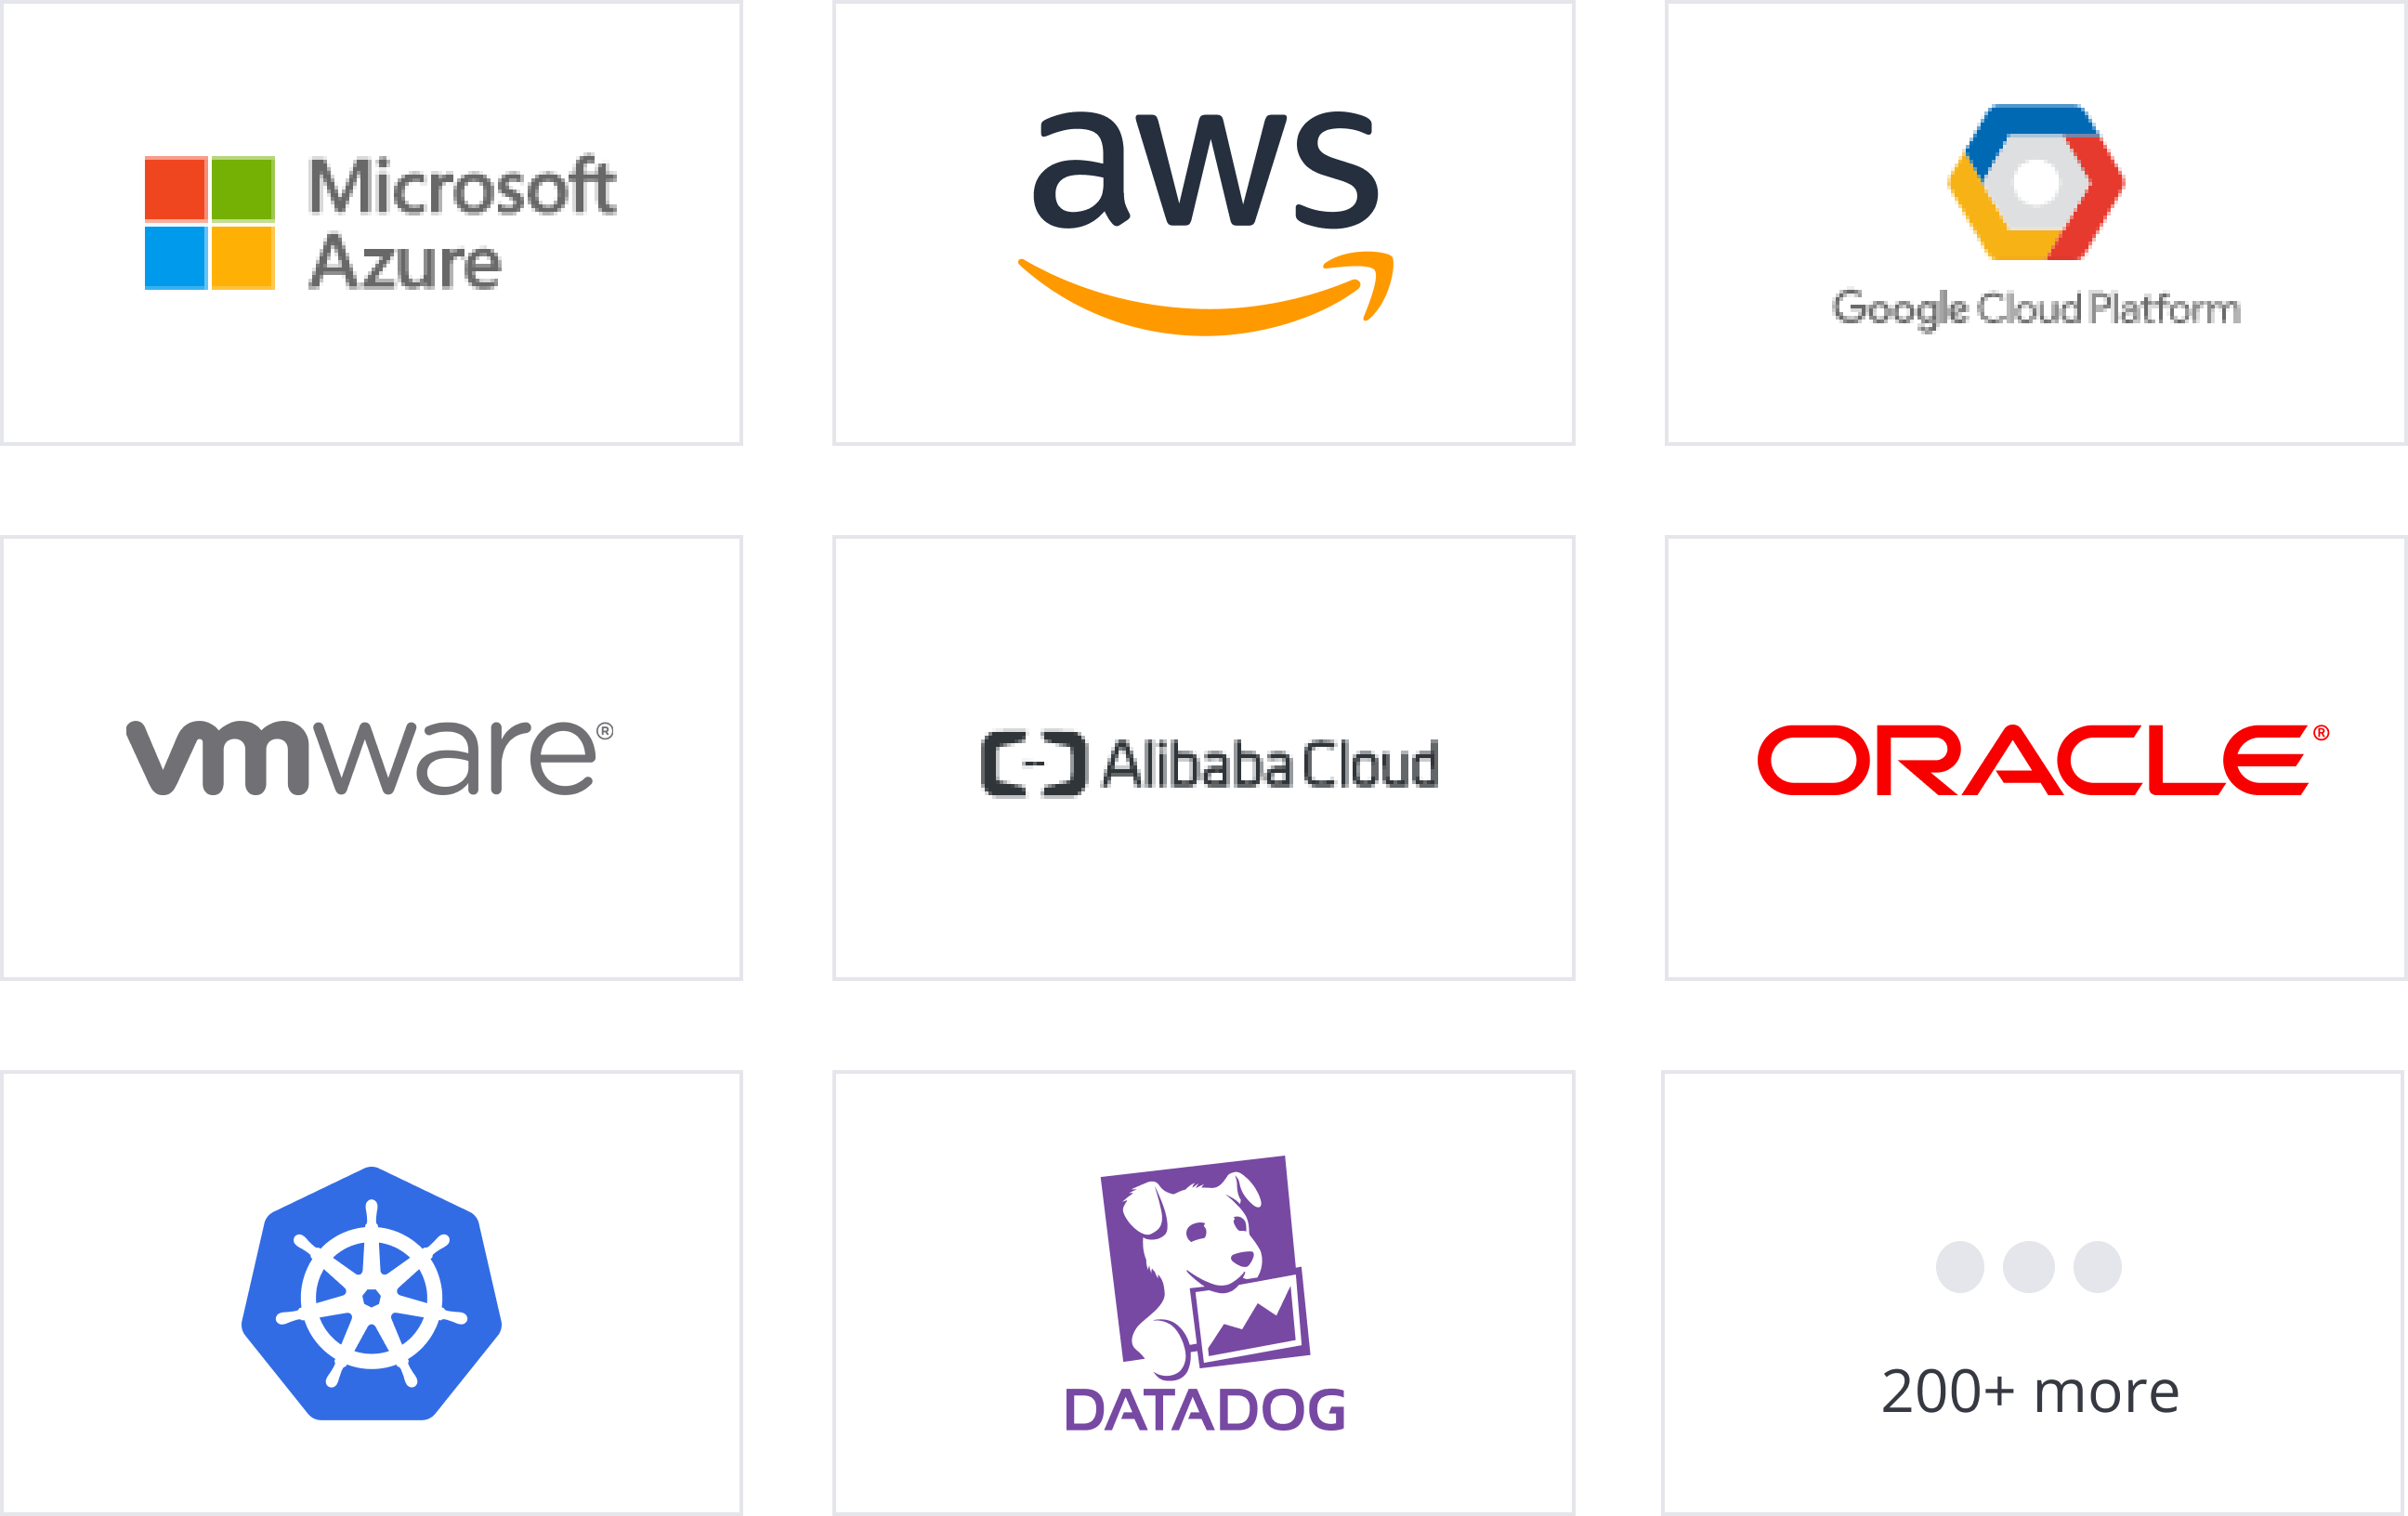
\includegraphics[width=0.55\linewidth]{images/TerraformProviders.png}	
\end{figure}

\paragraph{Serverless}
Serverless computing is a cloud computing execution model in which the cloud provider runs the server, and dynamically manages the allocation of machine resources. Pricing is based on the actual amount of resources consumed by an application, rather than on pre-purchased units of capacity \cite{serverless}. The benefits of this approach are the huge reduction in infrastructure and development expense. Engineers can focus on shipping their microservices and have secure, scalable infrastructure taken care of for them.
\\ \\
The Serverless Framework is also an example of IaC and provides developers with the ability to develop and deploy their serverless application to different cloud providers or simply Kubernetes (using \textbf{Knative}) if they wanted to run it on-premise or avoid code exposure to a cloud native service such as AWS Lambda or Google Cloud Functions.
\\ \\
This also provides quicker developer on-boarding and flexibility as a broad array of popular languages are supported. Given that the Function as a Service (\texttt{FaaS}) model is centred around the principles of loosely coupled microservices, this enables easy migration out of serverless architecture to a VM or container-based deployment. This may make sense in scenarios where there are cost savings to be made which typically applies to long-running, memory intensive tasks as opposed to short-lived and resource-light stateless services.

\begin{center}
\begin{tabular}{ p{5cm} p{5cm} }
	\toprule
	Provider & Supported Languages \\
	\midrule
	&\\
	AWS Lambda   & Python, Java, Go, Node, .NET, Ruby or Custom runtime  \\
	&\\
	Google Cloud Functions & Node, Python, Go and Java \\
	&\\
	Azure Functions & .NET, Node, Java, PowerShell and Python \\
	&\\
	IBM Cloud Functions & Node, Python, Swift, PHP, Go, Ruby, Java and .NET \\
	&\\
	Cloudflare Workers & JavaScript, TypeScript or Wasm-supported \\
	&\\
	\midrule
\end{tabular}
\end{center}

\paragraph{Open standards}
Open Standards allow people to share all kinds of data freely and with perfect fidelity. They prevent lock-in and other artificial barriers to interoperability, and promote choice between vendors and technology solutions. \cite{openstandards}

\subparagraph{OpenAPI}
The OpenAPI Specification (OAS) defines a standard, language-agnostic interface to RESTful APIs which allows both humans and computers to discover and understand the capabilities of the service without access to source code, documentation, or through network traffic inspection. When properly defined, a consumer can understand and interact with the remote service with a minimal amount of implementation logic. An OpenAPI definition can then be used by documentation generation tools to display the API, code generation tools to generate servers and clients in various programming languages, testing tools, and many other use cases. \cite{openapi}

\subparagraph{HL7 FHIR}
\textit{Fast Healthcare Interoperability Resources} (\texttt{FHIR}, pronounced "fire") is a standard describing data formats and elements (known as "resources") and an [API] for exchanging electronic health records (\texttt{EHR}). The standard was created by the Health Level Seven International (\texttt{HL7}) health-care standards organization. One of its goals is to facilitate interoperation between legacy health care systems, to make it easy to provide health care information to health care providers and individuals on a wide variety of devices from computers to tablets to cell phones, and to allow third-party application developers to provide medical applications which can be easily integrated into existing systems. \cite{fhir}

\subsection{Data ingestion}
\subsubsection{API management}
%TODO%
\paragraph{Authentication}
%TODO%
\paragraph{Gateway}
%TODO%

\begin{figure}[h!]
	\centering
	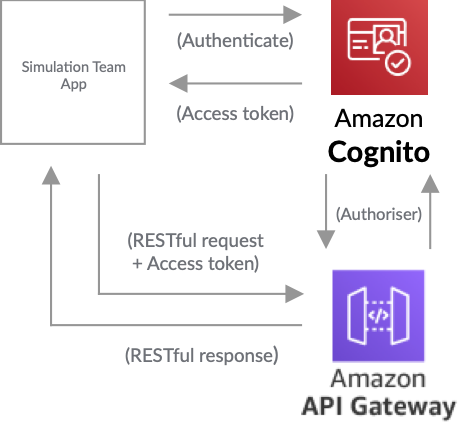
\includegraphics[width=0.4\linewidth]{images/APIGateway.png}	
	\caption*{Example: AWS API Gateway}
\end{figure}

\subsubsection{Microservices}
%TODO%

\begin{figure}[h!]
	\centering
	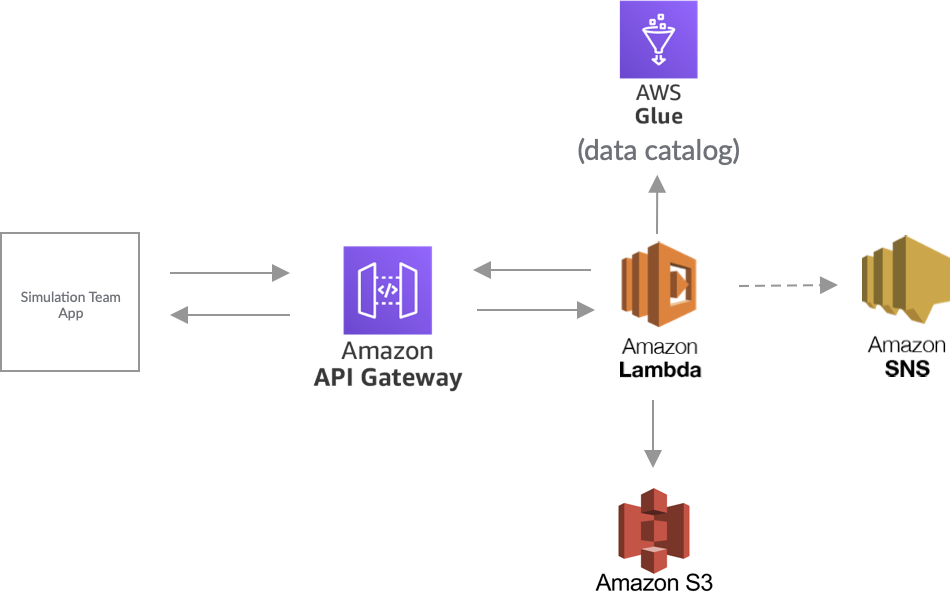
\includegraphics[width=0.6\linewidth]{images/Lambda.png}
	\caption*{Example: AWS Lambda}	
\end{figure}

\subsubsection{Metadata cataloguing}
\paragraph{Glue}
\subsubsection{Schema-less object store}
\paragraph{S3}

\subsection{Data warehousing}
\subsubsection{Federated querying}
\subsubsection{Common models}

\subsection{ETL \& data marts}
\subsubsection{Scheduling}
\subsubsection{Developers}
\subsubsection{Console}

\subsection{Secure access}
\subsubsection{Encryption}
Encryption is the process of turning plain text into a cipher, then using an encryption key to decrypt the cipher back to plain text.
\subsubsection{Concept}
Encryption is the process of turning plain text into a cipher, then using an encryption key to decrypt the cipher back to plain text.
\\
When data is received on the server to be encrypted it will require an encryption key to encrypt the data, this key is typically generated by either a key manager. When data is being retrieved or queried it will then use the same key to decrypt the data to be used.
\\
A key manager is used to generate, exchange, use, replace and delete cryptographic keys. It's able to deal with asymmetric and symmetric keys. Some key managers encrypt keys after generation to add another layer of security.
\\
Client-side encryption is an alternative option is to encrypt the data locally in the application before it gets to the server. This means the server is not involved in the cryptographic process of the data, as the application will use its own encryption key which the server cannot access. This is beneficial for the users as it provides them peace of mind.
\subsubsection{Solutions}
In cloud computing services “Microsoft Azure Data Lake Storage Gen1”, “Google Cloud” and “AWS” all provide options for the client and server-side encryption.
\subsubsection{Example}
We will be looking at AWS S3, AWS Redshift and AWS KMS for an example of the implementation of encryption of data lakes.
\\\\\textbf{AWS S3}\\
Server-side encryption uses three different modes of server-side encryption: SSE-S3, SSE-C, or SSE-KMS. The following will be an example of SSE-KMS.
\\
SSE-KMS enables the choice of a customer-managed CMK (customer master key) or the AWS managed CMK for Amazon S3 in the account. AWS KMS and Amazon S3 perform the following actions on encryption:
\begin{itemize}
  \item Amazon S3 requests a plaintext data key and a copy of the key encrypted under the specified CMK.
  \item AWS KMS generates a data key, encrypts it under the CMK and sends both the plaintext data key and the encrypted data key to Amazon S3.
  \item Amazon S3 encrypts the data using the data key and removes the plaintext key from memory as soon as possible after use.
  \item Amazon S3 stores the encrypted data key as metadata with the encrypted data.
\end{itemize}

Amazon S3 and AWS KMS perform the following actions when data is requested to be decrypted:
\begin{itemize}
    \item Amazon S3 sends the encrypted data key to AWS KMS.
    \item AWS KMS decrypts the key by using the same CMK and returns the plaintext data key to Amazon S3.
    \item Amazon S3 decrypts the ciphertext and removes the plaintext data key from memory as soon as possible.
\end{itemize}

Client-Side Encryption with AWS can use Amazon S3 Encryption Client in the AWS SDK of an application to encrypt objects and upload them to Amazon S3. This method ensures its security as it passes to the Amazon S3 service. The Amazon S3 service receives the encrypted data; it does not play a role in encrypting or decrypting it.
\\\\\textbf{AWS Redshift}\\
Amazon Redshift uses a four-tier, key-based architecture for encryption. The architecture consists of data encryption keys, a database key, a cluster key and a master key.
\\
Data encryption keys encrypt data blocks in the cluster. Each data block is assigned a randomly generated AES-256 key. These keys are encrypted by using the database key for the cluster.
\\
The database key encrypts data encryption keys in the cluster. The database key is a randomly generated AES-256 key. It is stored on disk in a separate network from the Amazon Redshift cluster and passed to the cluster across a secure channel.
\\
The cluster key encrypts the database key for the Amazon Redshift cluster.  AWS KMS, AWS CloudHSM, or an external hardware security module (HSM) can be used to manage the cluster key.
\\
The master key encrypts the cluster key. AWS KMS customer master key (CMK) can be used as the master key for Amazon Redshift.

\\\textbf{AWS KMS} \\
AWS Key Management Service (KMS) allows you to create and manage cryptographic keys and control their use across a wide range of AWS services and in the applications. AWS KMS uses hardware security modules that have been validated under FIPS 140-2, or are in the process of being validated, to protect keys. AWS KMS is integrated with AWS CloudTrail to provide logs of all key usage to help meet applicable regulatory and compliance needs.
\\
What is going on when S3 handles the process of server-side encryption:
\begin{itemize}
    \item When an object is upload into S3 and specify SSE, a unique 256-bit key (a data key) is generated and the data is encrypted using that key with AES-256.
    \\{images/KMSDiagram1.png}\\
    \item The data key is then encrypted using a master key, which S3 retrieves from KMS using the master key ID that was supplied in the s3 cp command.
    \\{images/KMSDiagram2.png}\\
    \item The encrypted data key is then stored with the encrypted data in the S3 bucket.
    \\{images/KMSDiagram3.png}\\
\end{itemize}
\\\textbf{Overview} \\
\\{images/EncryptionOverview.png}
The major steps in this process are
\begin{enumerate}
  \item You create a master key in AWS KMS
  \item You load the data into S3.
  \item S3 retrieves the key from KMS and encrypts the data.
  \item You run the COPY command in Amazon Redshift to load the data from S3.
\end{enumerate}
\subsubsection{IAM}
\subsubsection{Concept}
Identity and Access management (IMA) is used to make sure authorised users have the right to services while preventing access to non-authorised users guarantying secure access. It does this by defining and managing the roles, the access privileges of individual users and the circumstance users are granted those privileges.
\\
IAM allows access management over computing, storage, database and application services. It gives one identity per individual. Once that identity has been introduced, it must be maintained, modified and monitored throughout each user’s access lifecycle.
\subsubsection{Solutions}
Each cloud service provider offers a built an associated IAM. Independent IAM includes Okta Identity Cloud, JumpCloud and Auth0 which are all compatible with a range of cloud service providers.
\subsubsection{Examples}
We will be examining AWS Identity and Access Management. IAM is a feature of an AWS account offered at no additional charge. 
\\
The use cases of AWS IAM include finite-grained access control to AWS resources, Multifactor authentication for high privilege users, analyse access across the AWS environment and ability to integrate with the corporate directly (integration of current IAM system). 
\\\\\textbf{How it works} \\
AWS IAM allows us to:
\begin{itemize}
    \item Manage IAM users and their access –  Create users in IAM, assign them individual security credentials (access keys, passwords and multi-factor authentication devices), or request temporary security credentials to provide users access to AWS services and resources. Manage permissions in order to control which operations a user can perform.
    \item Manage IAM roles and their permissions – Create roles in IAM and manage permissions to control which operations can be performed by the entity, or AWS service, that assumes the role. Define which entity can assume the role. In addition, you can use service-linked roles to delegate permissions to AWS services that create and manage AWS resources automatically.
    \item Manage federated users and their permissions – Enable identity federation to allow existing identities (users, groups and roles) in the enterprise to access the AWS Management Console, call AWS APIs and access resources, without the need to create an IAM user for each identity. Enable the use of any identity management solution that supports SAML 2.0.
\end{itemize}
\subsubsection{Logging}
\subsubsection{Concept}
A Log is data that can describe application information, system performance and user activity, for example, might include Timestamp, Application, User, Session ID .etc.
\\
Using logs to monitor the use of the system provides security to check for violations and unpredicted behaviour from users and the system. Analysing, searching and filtering logs discovers and alerts these incidents. It enables access to historic information for debugging and forensic investigations.
\subsubsection{Examples}
The example which will show the use of logs is Amazon CloudWatch Logs. Amazon CloudWatch Logs can be used to monitor, store and access the log files from AWS Services. AWS Identity and Access Management (IAM) and AWS Lambda used in conjunction with CloudWatch Logs.
\\
CloudWatch Logs enables the centralization of the logs from all over the systems, applications and AWS services that are used, in a single, highly scalable service. You can then easily view them, search them for specific error codes or patterns, filter them based on specific fields, or archive them securely for future analysis. 
\\\\\textbf{Features} \\
Query the Log Data – CloudWatch Logs Insights can be used to interactively search and analyse log data. CloudWatch provides sample queries, command descriptions, query autocompletion and log field discovery to help get started. 
\\
Monitor AWS CloudTrail Logged Events – You can create alarms in CloudWatch and receive notifications of particular API activity as captured by CloudTrail and use the notification to perform troubleshooting.
\\
Log Retention – By default, logs are kept indefinitely and never expire. You can adjust the retention policy for each log group, keeping the indefinite retention, or choosing a retention period between 10 years and one day.
\\
Archive Log Data – CloudWatch Logs can be used to store log data in highly durable storage. The CloudWatch Logs agent makes it easy to quickly send both rotated and non-rotated log data off of a host and into the log service. You can then access the raw log data when needed.
\newpage
\section{Development Testing}
\subsection{Local environment}
\subsubsection{API development}
%TODO%
\paragraph{Serverless}
The Serverless Framework enables developers to run an emulated environment locally instead of needing to deploy that serverless app for testing. This comes with over 1,000 plugins that can emulate services such as AWS Lambda and API Gateway. 
\paragraph{Postman}

Postman is a very popular tool used by developers that want to conveniently test and build APIs in a collaborative way.
\\ \\
As we are implementing the OpenAPI specification, Postman enables the import of Swagger files to automatically generate a Postman environment. This makes developer on-boarding much easier as versioned mock endpoints and documentation are hosted for us as part of the DevOps deployment.


\subsection{DevOps pipeline}
\subsubsection{GitHub}
\subsubsection{CircleCI}
\subsubsection{CodeDeploy}

\section{Release Testing}
\subsection{Staging}
\subsection{Production}

\newpage
\section{OO Design \& UML}
\newpage

\printbibliography

\end{document}
